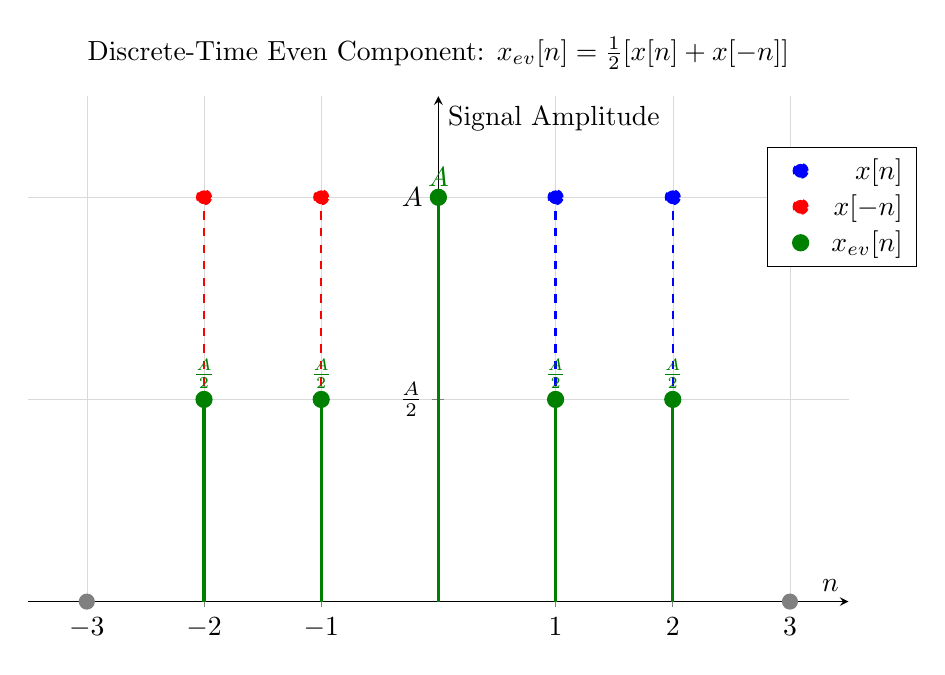
\begin{tikzpicture}
	% Define styles for the different stem plots
	\pgfplotsset{
		impulse/.style={ ycomb, thick, mark=*, mark size=2.5pt },
		original/.style={ impulse, blue, dashed },
		reversed/.style={ impulse, red, dashed },
		even/.style={ impulse, green!50!black, very thick },
	}
	
	\begin{axis}[
		% Set the overall style
		width=12cm,
		height=8cm,
		% Title with the definition of the even component
		title={Discrete-Time Even Component: $x_{ev}[n] = \frac{1}{2}[x[n] + x[-n]]$},
		% Axis labels
		xlabel={$n$},
		ylabel={Signal Amplitude},
		% Position axes at the origin
		axis lines=middle,
		% Set axis limits
		xmin=-3.5, xmax=3.5,
		ymin=0, ymax=2.5,
		% Set ticks at key points
		xtick={-3, -2, -1, 0, 1, 2, 3},
		ytick={1, 2},
		yticklabels={$\frac{A}{2}$, $A$},
		% Add a grid
		grid=major,
		grid style={line width=.1pt, draw=gray!30},
		% Position the legend
		legend style={
	at={(0.9, 0.9)}, % 3% from left, 97% from bottom
	anchor=north west,   % Anchor the top-left corner of the legend
	legend cell align={right}
},
		]
		
		% 1. Plot the original signal (dashed blue)
		\addplot[original] coordinates {(0,2) (1,2) (2,2)};
		\addlegendentry{$x[n]$};
		
		% 2. Plot the time-reversed signal (dashed red)
		\addplot[reversed] coordinates {(-2,2) (-1,2) (0,2)};
		\addlegendentry{$x[-n]$};
		
		% 3. Plot the resulting even component (solid green)
		% Plot the A/2 components with their label
		\addplot[
		even,
		nodes near coords={$\frac{A}{2}$},
		every node near coord/.style={anchor=south, font=\footnotesize},
		] coordinates {(-2,1) (-1,1) (1,1) (2,1)};
		\addlegendentry{$x_{ev}[n]$};
		
		% Plot the A component separately to give it the correct label
		\addplot[even, nodes near coords={$A$}, every node near coord/.style={anchor=south}] 
		coordinates {(0,2)};
		
		% Plot some zero-value points for context
		\addplot[impulse, gray] coordinates {(-3,0) (3,0)};
		
	\end{axis}
\end{tikzpicture}